\section{Verfahrensbeschreibung}
\label{sec:verfahrensbeschreibung}

% Allgemeine Verfahrensbeschreibung
Für den zu simulierenden Sachverhalt lohnt es sich, jede Bewegung der Kamera in Phasen zu unterteilen, um unübersichtliche Strukturen zu vermeiden.
So bietet es sich an, eine \emph{Phase} (\texttt{Phase}) als entweder eine \emph{Beschleunigungs-} (\texttt{ACCELERATION}), \emph{Konstantgeschwindigkeits-} (\texttt{CONSTANT\_VELOCITY}) oder eine \emph{Bremsphase} (\texttt{DECELERATION}) zu definieren.

Eine \emph{Bewegung} (\texttt{Movement}) besteht dann aus entweder einer Beschleunigungs-, einer Konstantgeschwindigkeits- und einer Bremsphase oder nur aus einer Beschleunigungs- und einer Bremsphase.

Eine Instanz der Spidercam (\texttt{Spidercam}) enthält dann zusätzlich zu bekannten Konstanten $v_{\max}$ (\texttt{max\_velocity}) und $a_{\max}$ (\texttt{acceleration}) eine Liste von Bewegungen (\texttt{movements}) und eine einelementige Warteschlange (\texttt{queue}).
Zusätzlich kennt die Spidercam ihre initiale Position (\texttt{start}).

\subsection{Datenstrukturen}
\label{ssec:datenstrukturen}

% Beschreibung der Datenstrukturen

\subsubsection{Phase}
\label{sssec:phase}

Eine Phase (\texttt{Phase}) wird als eine Klasse modelliert, die eindeutig durch folgende Attribute definiert ist:
\begin{itemize}
    \item \texttt{movement}: Eine Referenz auf die Bewegung, zu der die Phase gehört.
    \item \texttt{mode}: Ein Wert aus dem Enum \texttt{Mode}, der angibt, ob es sich um eine Beschleunigungs- (\texttt{ACCELERATION}), Konstantgeschwindigkeits- (\texttt{CONSTANT\_VELOCITY}) oder Bremsphase (\texttt{DECELERATION}) handelt.
    \item \texttt{start}: Startkoordinaten der Phase.
    \item \texttt{starting\_velocity}: Startgeschwindigkeit der Phase.
    \item \texttt{dest}: Endkoordinaten der Phase.
\end{itemize}

Nachdem eine Phase mit den genannt Attributen initialisiert wurde, kann mithilfe der Funktion \texttt{update()} die Phase aktualisiert werden.
Dabei wird abhängig vom Modus der Phase berechnet, welche Distanz (\texttt{distance}) am Ende der Phase zurückgelegt wurde und wie lange die Phase dauert (\texttt{duration}).


\begin{figure}[H]
    \centering
    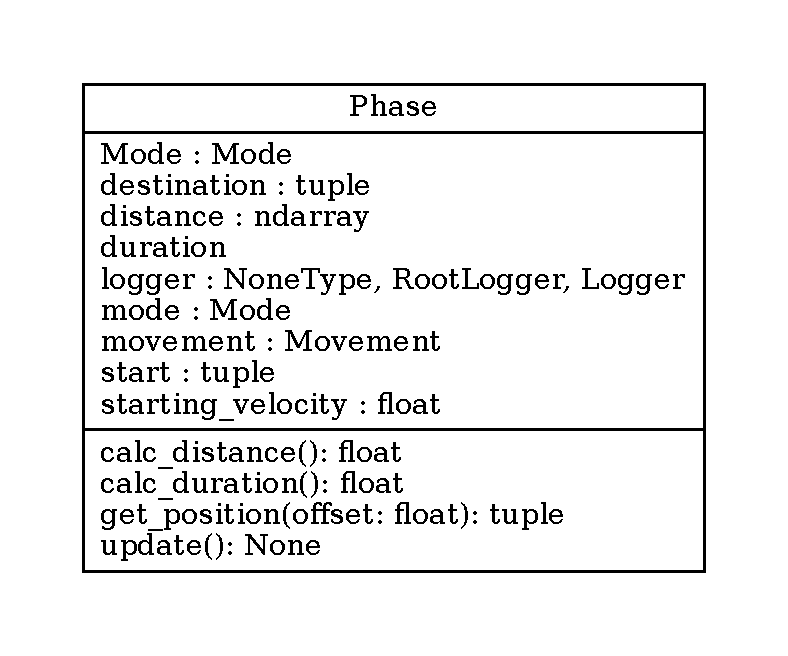
\includegraphics[width=0.7\textwidth]{../python/uml/phase.pdf}
    \caption{Klassendiagramm der Klasse \texttt{Phase}}
    \label{fig:phase}
\end{figure}

\subsubsection{Movement}
\label{sssec:movement}

Eine Bewegung (\texttt{Movement}) wird als eine Klasse modelliert, die eindeutig durch folgende Attribute definiert ist:
\begin{itemize}
    \item \texttt{spidercam}: Eine Referenz auf die Spidercam, zu der die Bewegung gehört.
    \item \texttt{start\_time}: Startzeitpunkt der Bewegung.
    \item \texttt{start}: Startkoordinaten der Bewegung.
    \item \texttt{destination}: Endkoordinaten der Bewegung.
\end{itemize}

Nachdem eine Bewegung mit den genannten Attributen initialisiert wurde, können mithilfe der Funktion \texttt{calculate\_phases()} die Phasen der Bewegung berechnet werden.
Diese werden dann in der Liste \texttt{phases} gespeichert.

Die Start- und Endkoordinaten der Bewegung können mithilfe der Funktionen \texttt{start()} und \texttt{dest()} abgerufen werden.
Dabei werden die Startkoordinaten der ersten bzw. die Endkoordinaten der letzten Phase zurückgegeben.

\begin{figure}[H]
    \centering
    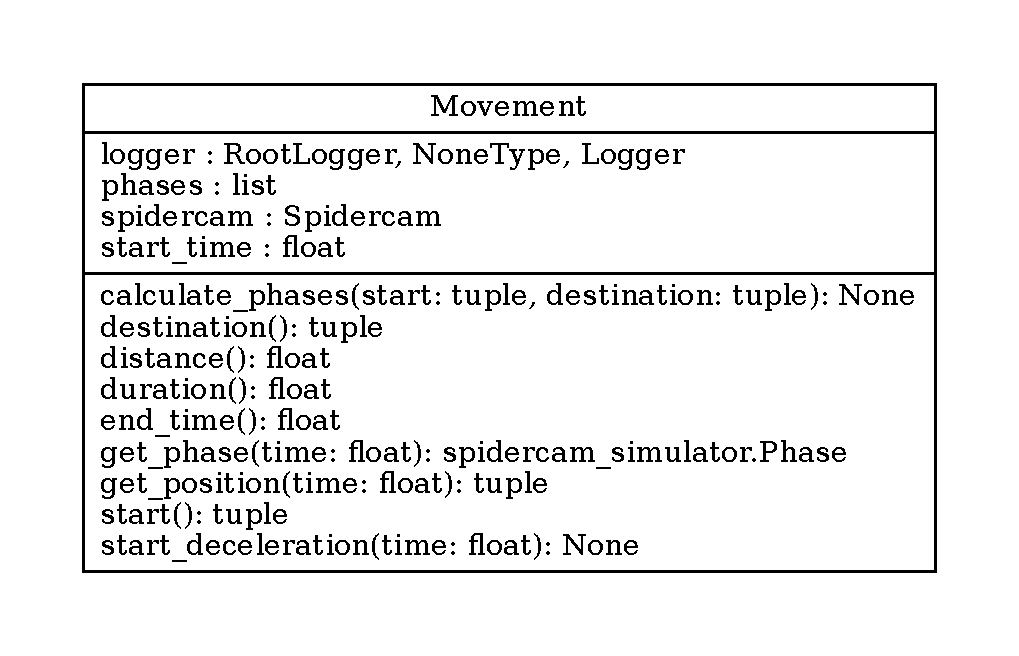
\includegraphics[width=0.7\textwidth]{../python/uml/movement.pdf}
    \caption{Klassendiagramm der Klasse \texttt{Movement}}
    \label{fig:movement}
\end{figure}

\subsubsection{Spidercam}
\label{sssec:spidercam}

Eine Spidercam (\texttt{Spidercam}) wird als eine Klasse modelliert, die eindeutig durch folgende Attribute definiert ist:
\begin{itemize}
    \item \texttt{controller}: Eine Referenz auf den Controller, zu dem die Spidercam gehört.
    \item \texttt{max\_velocity}: Maximale Geschwindigkeit der Spidercam.
    \item \texttt{acceleration}: Beschleunigung der Spidercam.
    \item \texttt{start}: Startkoordinaten der Spidercam.
\end{itemize}

Nachdem eine Spidercam mit den genannten Attributen initialisiert wurde, können mithilfe der Funktion \texttt{calc\_constants()} weitere Konstanten der Bewegung berechnet werden.
Diese sind konkret wie in \ref{ssec:mathematische_modellierung} beschrieben $t_{\max}$ (\texttt{time\_vmax}) und $d_{\max}$ (\texttt{distance\_vmax}).

\begin{figure}[H]
    \centering
    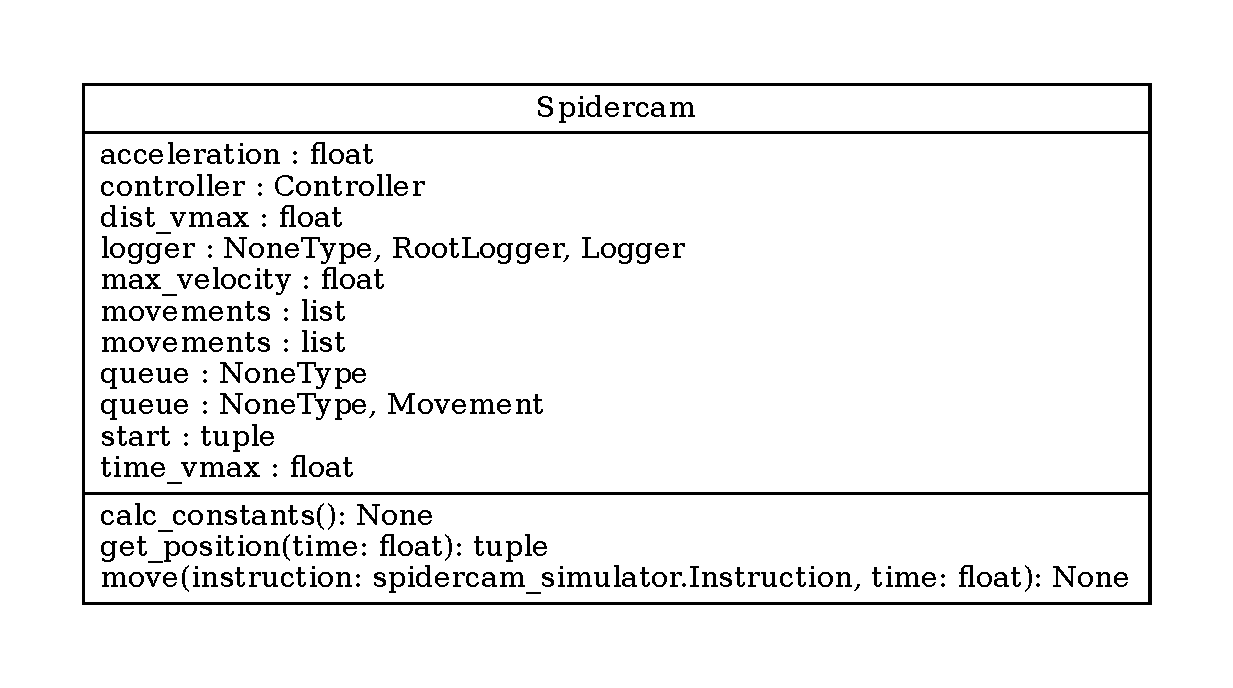
\includegraphics[width=0.7\textwidth]{../python/uml/spidercam.pdf}
    \caption{Klassendiagramm der Klasse \texttt{Spidercam}}
    \label{fig:spidercam}
\end{figure}

\subsubsection{Controller}
\label{sssec:controller}

Um die Bewegungen der Spidercam zu steuern, wurde ein Controller (\texttt{Controller}) implementiert.
Dieser wird als eine Klasse modelliert, die eindeutig durch folgende Attribute definiert ist:
\begin{itemize}
    \item \texttt{dim}: Dimension des Raumes, in dem sich die Spidercam bewegt.
    \item \texttt{start}: Startkoordinaten der Spidercam.
    \item \texttt{max\_velocity}: Maximale Geschwindigkeit der Spidercam.
    \item \texttt{acceleration}: Beschleunigung der Spidercam.
    \item \texttt{freq}: Diskretisierungsfrequenz der Bewegung.
    \item \texttt{instructions}: Liste der Bewegungsanweisungen.
\end{itemize}

Nachdem der Controller mit den genannten Attributen initialisiert wurde, berechnet dieser mithilfe der Funktion \texttt{calc\_anchors()} die fixen Ankerpunkte der Drahtseile.
Diese werden in der Liste \texttt{anchors} gespeichert.

Anschließend kann der Controller  mit der Funktion \texttt{run()} gestartet werden.
Dabei wird in diskreten Zeitintervallen der Frequenz \texttt{freq} die Spidercam entweder mit einer neuen Instruktion beauftragt, wenn eine noch nicht bearbeitete Instruktion zum aktuellen Zeitpunkt existiert, oder die Spidercam zum aktuellen Zeitpunkt aktualisiert.
In jedem Zeitpunkt wird die aktuelle Position der Spidercam bestimmt und damit die aktuellen Längen der Drahtseile berechnet.
Diese werden dann in den Listen \texttt{cam\_positions} und \texttt{rope\_lengths} gespeichert.

\begin{figure}[H]
    \centering
    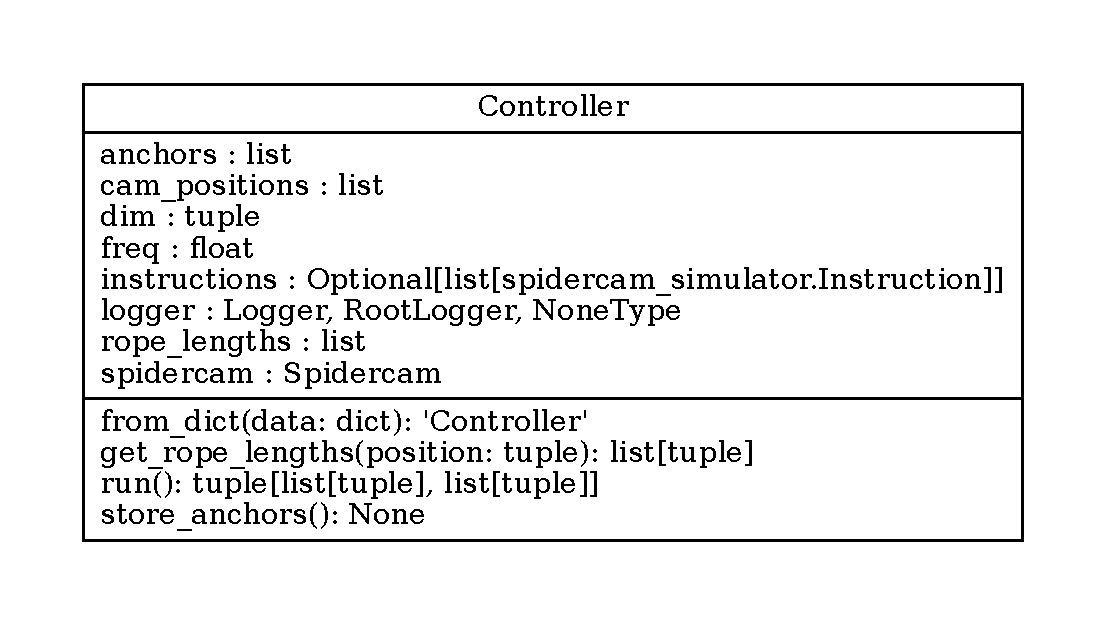
\includegraphics[width=0.7\textwidth]{../python/uml/controller.pdf}
    \caption{Klassendiagramm der Klasse \texttt{Controller}}
    \label{fig:controller}
\end{figure}

\subsubsection{Input und Output}
\label{sssec:helper}

Um insbesondere den Import von Eingabedateien und den Export von Ausgabedateien zu vereinfachen, wurden einige Hilfsklassen und -funktionen implementiert.

\paragraph{FileHandler}
\label{sssec:filehandler}

Die Klasse \texttt{FileHandler} ist eine Hilfsklasse, die zu einer Eingabedatei die entsprechenden Ausgabedateien erzeugt.
Diese wird instanziiert, indem ihr die Pfade zur Eingabe\emph{datei} und zum Ausgabe\emph{ordner} übergeben werden.
Basierend auf dem Namen der Eingabedatei werden dann die Pfade zu den Ausgabedateien bzw. die Ausgabedateien selbst definiert.

\paragraph{Instruction}
\label{sssec:instruction}

Die Klasse \texttt{Instruction} ist eine Hilfsklasse, die eine Bewegungsanweisung repräsentiert.
Diese wird instanziiert, indem ihr eine syntaktisch korrekte Zeile aus einer Eingabedatei übergeben wird, in der die Bewegungsanweisung definiert ist.
Die Instanz enthält dann den definierten Startzeitpunkt der Bewegungsanweisung (\texttt{start\_time}) und das Ziel der Bewegungsanweisung (\texttt{destination}).

\paragraph{Parser}
\label{sssec:parser}

Die Klasse \texttt{Parser} ist eine Hilfsklasse, die eine Eingabedatei einliest und die darin definierten Parameter und Bewegungsanweisungen extrahiert.
Die statische Methode \texttt{parse\_input()} dieser Klasse erwartet als Parameter einen String, der den Inhalt einer Eingabedatei enthält.
Die Methode erzeugt dann ein Dictionary mit den extrahierten Parametern und Bewegungsanweisungen und gibt dieses zurück.

Die ebenfalls statische Methode \texttt{parse\_output()} dieser Klasse erwartet als Parameter die folgenden zu exportierenden Daten:
\begin{itemize}
    \item Für Ausgabedatei 1:
          \begin{itemize}
              \item \texttt{rope\_lengths}: Liste der Längen der Drahtseile in jedem Zeitpunkt.
          \end{itemize}
    \item Für Ausgabedatei 2:
          \begin{itemize}
              \item \texttt{dim}: Dimension des Raumes, in dem sich die Spidercam bewegt.
              \item \texttt{freq}: Diskretisierungsfrequenz der Bewegung.
              \item \texttt{cam\_positions}: Liste der Positionen der Spidercam in jedem Zeitpunkt.
          \end{itemize}
\end{itemize}

Entsprechend des in \ref{ssec:ausgabe} definierten Ausgabeformats werden die Daten in zwei Strings umgewandelt und zurückgegeben.

\begin{figure}[H]
    \centering
    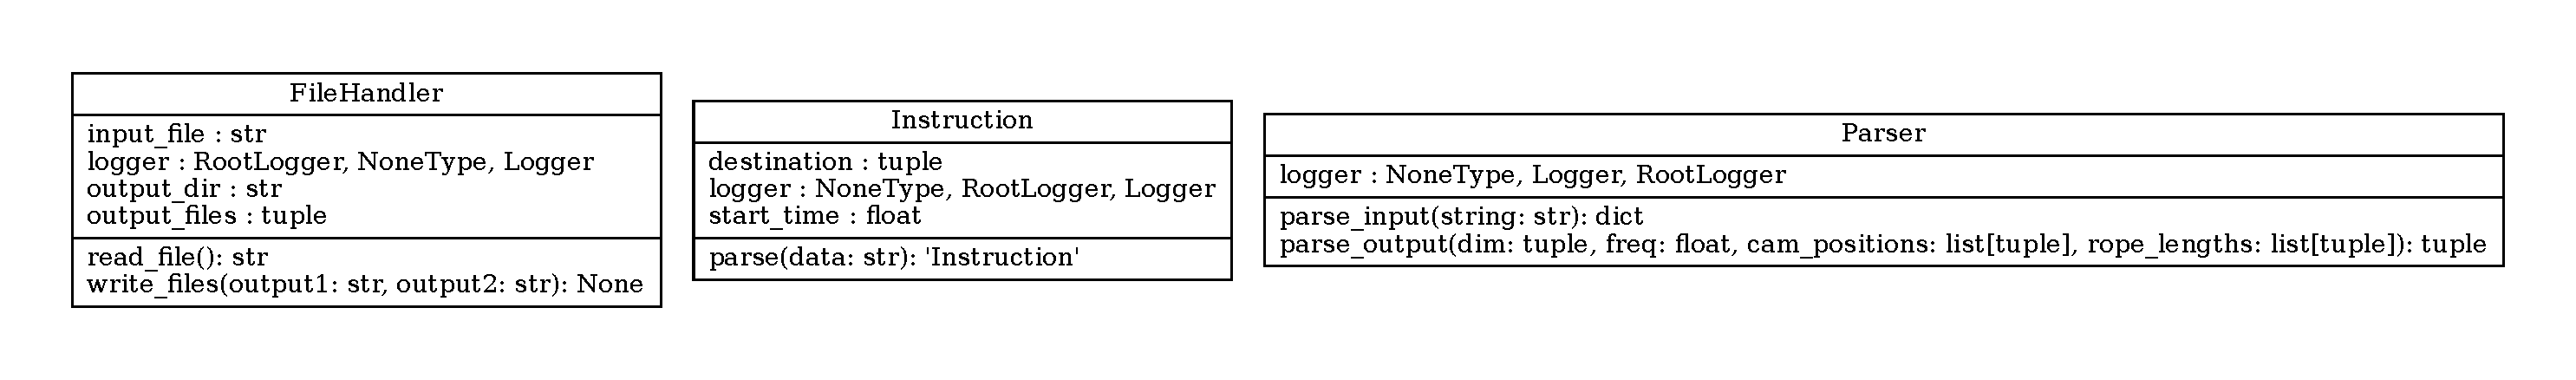
\includegraphics[width=\textwidth]{../python/uml/io.pdf}
    \caption{Klassendiagramme der Hilfsklassen \texttt{FileHandler}, \texttt{Instruction} und \texttt{Parser}}
    \label{fig:io}
\end{figure}

\subsubsection{Plotter}
\label{ssec:plotter}

Auf diese Klasse soll hier nur kurz eingegangen werden.
Sie ist eine Hilfsklasse, die die Ausgabedateien 1 und 2 in Form von Graphen visualisiert.
Diese wird instanziiert, indem ihr analog zur Funktion \texttt{parse\_output()} die entsprechenden Daten übergeben werden.

\begin{figure}[H]
    \centering
    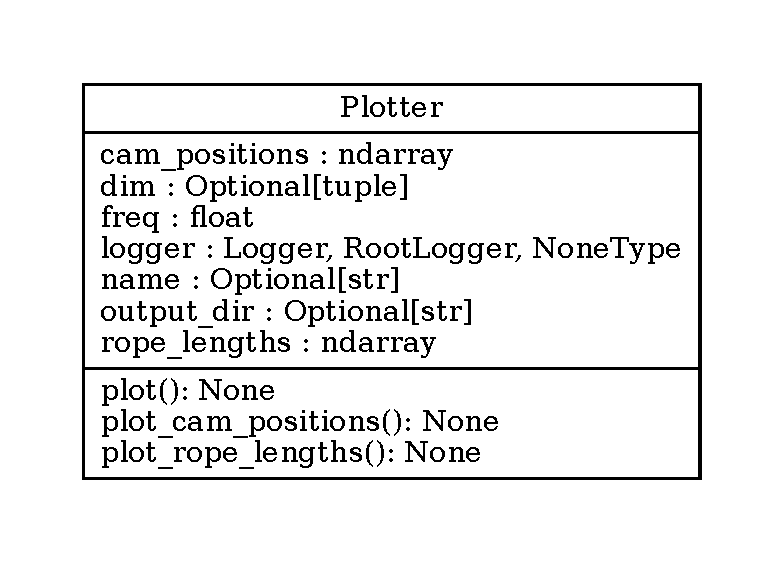
\includegraphics[width=0.7\textwidth]{../python/uml/plotter.pdf}
    \caption{Klassendiagramm der Klasse \texttt{Plotter}}
    \label{fig:plotter}
\end{figure}

\subsection{Algorithmen}
\label{ssec:algorithmen}

% Beschreibung der Algorithmen
Die genutzten Algorithmen unterteilen sich in drei Kategorien:
\begin{itemize}
    \item Verarbeitung der Eingabedatei
    \item Bewegung der Spidercam
    \item Erstellung der Ausgabedatei
\end{itemize}

\subsubsection{Verarbeitung der Eingabedatei}
\label{sssec:verarbeitung_der_eingabedatei}

% Beschreibung der Verarbeitung der Eingabe
Die Eingabe wird wie bereits definiert in der Funktion \texttt{parse\_input()} der Klasse \texttt{Parser} verarbeitet.

Der Eingabestring wird Zeile für Zeile durchlaufen und die Zeilen werden anhand der ersten Zeichen der Zeilen der jeweiligen Kategorie (\texttt{dim}, \texttt{start}, $\ldots$) zugeordnet.

Anschließend werden die einzelnen Parameter auf ihre semantische Korrektheit überprüft (siehe dazu die definierten Fehlerquellen in \ref{sssec:fehlerquellen_und_-behebung}).
Sind alle Parameter korrekt, wird ein Dictionary mit den extrahierten Parametern und Bewegungsanweisungen zurückgegeben.

Für eine Visualisierung siehe Abbildung \ref{fig:parse_input}.

\begin{figure}[H]
    \centering
    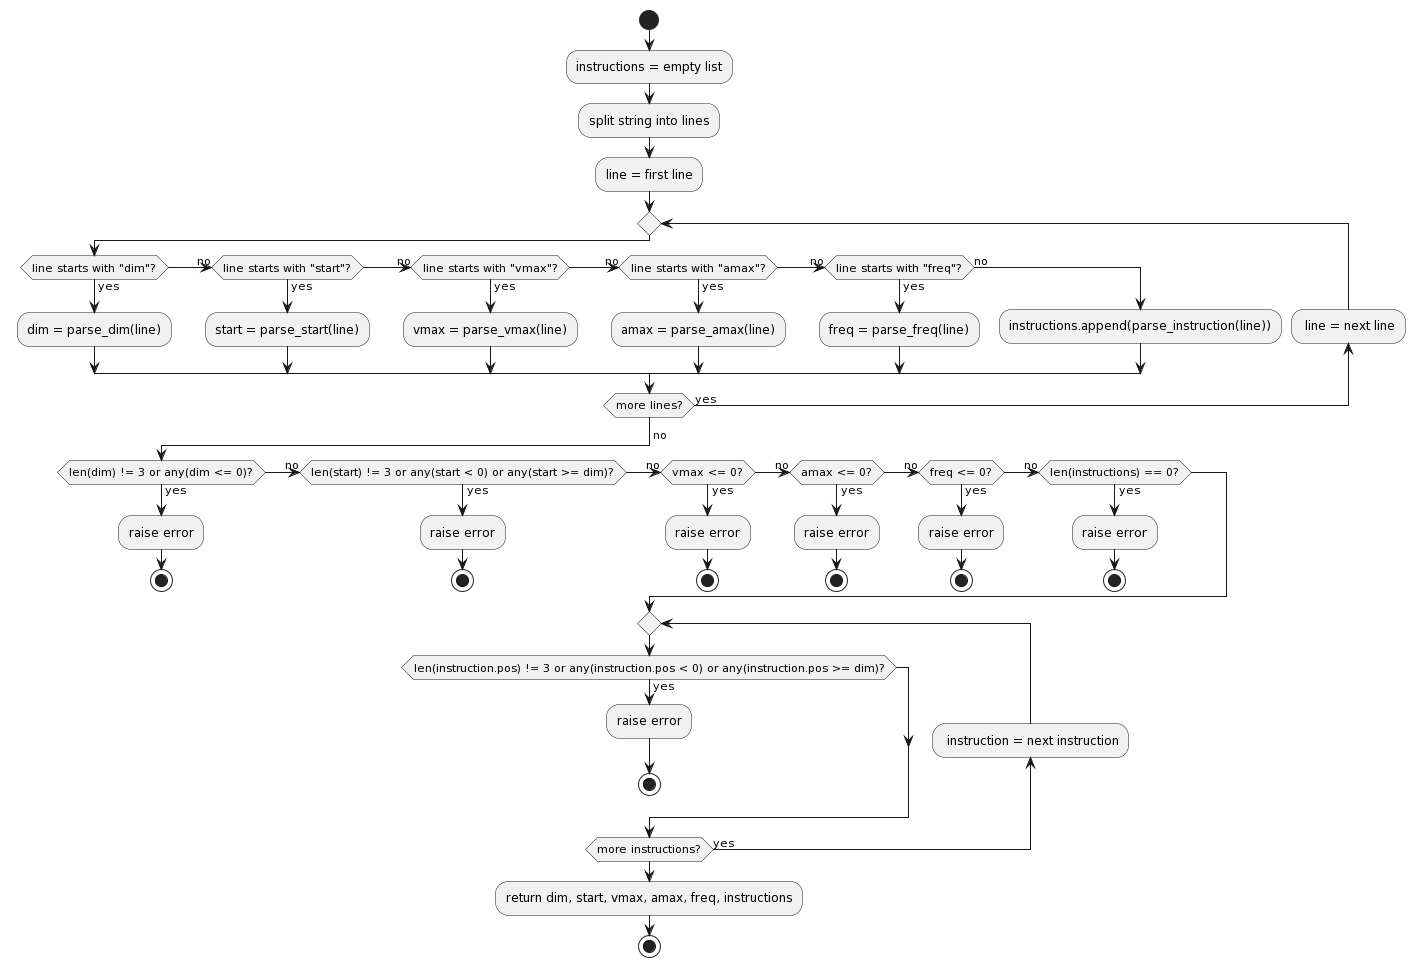
\includegraphics[width=\textwidth]{../python/uml/activity_parse_input.png}
    \caption{Aktivitätsdiagramm der Funktion \texttt{parse\_input()} der Klasse \texttt{Parser}}
    \label{fig:parse_input}
\end{figure}

\subsubsection{Bewegung der Spidercam}
\label{sssec:bewegung_der_spidercam}

% Beschreibung der Bewegung der Spidercam
Die Bewegung der Spidercam wird in der Funktion \texttt{move()} der Klasse \texttt{Spidercam} durchgeführt.
Dabei kann zwischen zwei Fällen unterschieden werden:
\begin{enumerate}
    \item Die Spidercam bekommt eine neue Bewegungsanweisung \texttt{instruction}, siehe \ref{sssec:neue_bewegungsanweisung}.
    \item Die Spidercam erhält einen Zeitpunkt \texttt{time} und soll für diesen aktualisiert werden, siehe \ref{sssec:aktualisierung_fuer_zeitpunkt}.
\end{enumerate}

\begin{figure}[H]
    \centering
    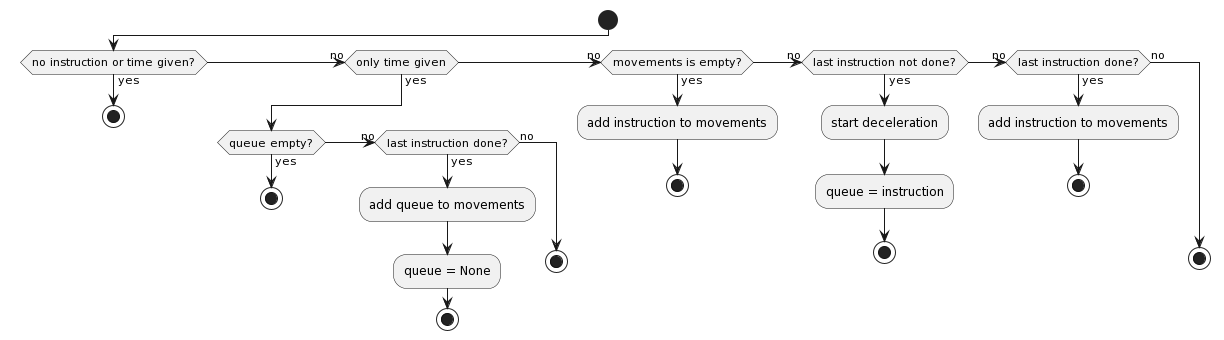
\includegraphics[width=\textwidth]{../python/uml/activity_move.png}
    \caption{Aktivitätsdiagramm der Funktion \texttt{move()} der Klasse \texttt{Spidercam}}
    \label{fig:move}
\end{figure}

\paragraph{Neue Bewegungsanweisung}
\label{sssec:neue_bewegungsanweisung}
% Beschreibung der Bewegung der Spidercam bei einer neuen Bewegungsanweisung
Wird der Spidercam eine neue Bewegungsanweisung \texttt{instruction} übergeben, so wird die übergebene Instruktion als neues \texttt{Movement} in der Liste \texttt{movements} der Spidercam gespeichert, wenn entweder noch keine Bewegung stattgefunden hat (\texttt{movements} ist leer) oder die letzte Bewegung bereits abgeschlossen ist (\texttt{movements}[-1].\texttt{end\_time()} ist kleiner als \texttt{time}).
Der Startpunkt der Bewegung ist dabei also entweder das Ziel der letzten Bewegung oder die Startposition der Spidercam.

Andernfalls wird zum Zeitpunkt \texttt{time} der Bremsvorgang eingeleitet (siehe \ref{sssec:bremsvorgang}) und die aktuelle Warteschlange \texttt{queue} überschrieben.

\paragraph{Aktualisierung für Zeitpunkt}
\label{sssec:aktualisierung_fuer_zeitpunkt}

% Beschreibung der Bewegung der Spidercam bei einer Aktualisierung für einen Zeitpunkt
Wird der Spidercam ein Zeitpunkt \texttt{time} übergeben, so wird überprüft, ob die aktuelle Bewegung abgeschlossen ist.
Ist dies der Fall, wird, sofern vorhanden, die nächste Bewegung aus der Warteschlange \texttt{queue} in die Liste \texttt{movements} übernommen und die Warteschlange wird geleert.

Ist die aktuelle Bewegung noch nicht abgeschlossen, so muss nichts weiter getan werden.

\paragraph{Bremsvorgang}
\label{sssec:bremsvorgang}

% Beschreibung des Bremsvorgangs
Der Bremsvorgang wird mittels der Funktion \texttt{start\_deceleration()} der Klasse \texttt{Movement} eingeleitet, wenn die Spidercam eine neue Bewegungsanweisung erhält, die mit der aktuellen Bewegung kollidiert.

Dabei wird zuerst geprüft, in welche Bewegungsphase der aktuelle Zeitpunkt \texttt{time} fällt und wie viel Zeit in der Phase vergeht (\texttt{offset}).
In einer Bremsphase muss nichts weiter getan werden, da die Spidercam bereits abgebremst wird.

Andernfalls wird zunächst bestimmt, welcher Weg zum Zeitpunkt seit Beginn der Phase zurückgelegt und welcher Punkt erreicht wurde.
Dieser Punkt ist dann der Zielpunkt für die unterbrochene Phase und der Startpunkt der neuen Bremsphase.

Anschließend wird die neue Bremsphase so abgeändert, dass die Startgeschwindigkeit (\texttt{starting\_velocity}) der Bremsphase gleich der aktuellen Geschwindigkeit der Spidercam ist (siehe \ref{ssec:mathematische_modellierung}) und der Modus der Bremsphase auf \texttt{DECELERATION} gesetzt wird.
Es ist trivial, dass nach $v(t) \cdot a_{\max}^{-1}$ Sekunden die Geschwindigkeit der Spidercam 0 ist.
Der Zielpunkt der Bremsphase ist also eben dieser Punkt, der nach $v(t) \cdot a_{\max}^{-1}$ Sekunden während der Bremsphase erreicht wird.

\subsubsection{Erstellung der Ausgabedatei}
\label{sssec:erstellung_der_ausgabedatei}

% Beschreibung der Erstellung der Ausgabe
Nach \ref{ssec:ausgabe} sollen pro Eingabe zwei Ausgabedateien erstellt werden.
Diese Aufgabe wird in der Funktion \texttt{parse\_output()} der Klasse \texttt{Parser} durchgeführt.
Diese erhält als Parameter die Dimension des Raumes, die Diskretisierungsfrequenz und die Listen der Kamerapositionen und der Seillängen zu jedem Zeitpunkt.

Die erste Datei soll die Längen der Drahtseile zu jedem diskreten Zeitpunkt enthalten.
Dazu wird zunächst die Liste \texttt{rope\_lengths} transponiert, da pro Zeile die Längen eines einzelnen Seils auszugeben sind und die Liste \texttt{rope\_lengths} pro Zeile die Längen \emph{aller} Seile zu einem Zeitpunkt enthält.
Transponieren erzeugt also aus einer $n \times 4$-Matrix eine $4 \times n$-Matrix, durch deren Zeilen dann iteriert werden kann.
Dies erfolgt wie in Listing \ref{lst:parse_output1} beschrieben.

Die zweite Datei soll die Dimension, die diskreten Zeitpunkte und die Kamerapositionen zu jedem Zeitpunkt enthalten.
Analog zu den Seillängen wird auch hier zunächst die Liste \texttt{camera\_positions} transponiert, um pro Zeile eine Koordinate der Kameraposition zu erhalten.
Der Rest der Ausgabe erfolgt analog zu Listing \ref{lst:parse_output1}.

\begin{figure}[H]
    \centering
    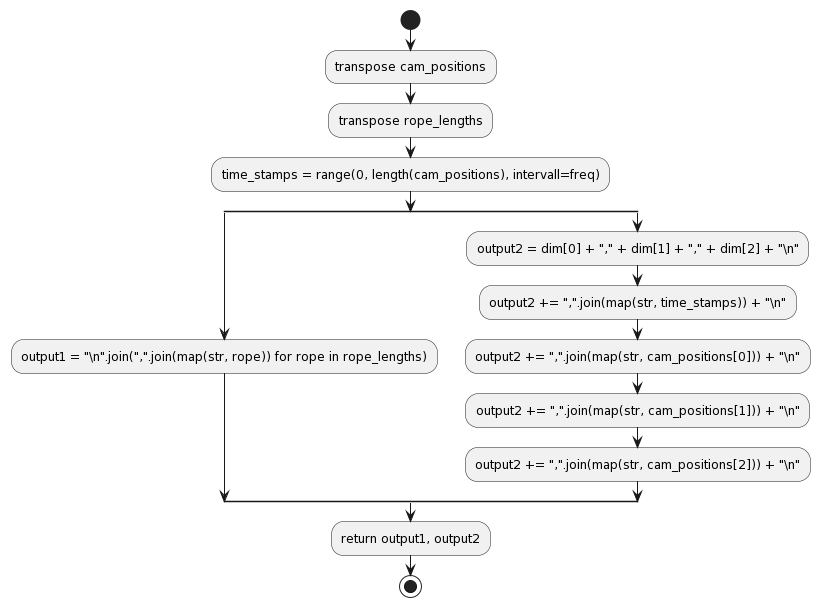
\includegraphics[width=0.8\textwidth]{../python/uml/activity_parse_output_simplified.png}
    \caption{Aktivitätsdiagramm der Funktion \texttt{parse\_output()}}
    \label{fig:activity_parse_output}
\end{figure}

\begin{lstlisting}[caption={Erstellung der Ausgabedatei 1 (Längen der Drahtseile)}, label={lst:parse_output1}, language=Python]
    output1 = "\n".join(",".join(map(str, rope)) for rope in rope_lengths)
\end{lstlisting}

\begin{lstlisting}[caption={Erstellung der Ausgabedatei 2 (Kamerapositionen)}, label={lst:parse_output2}, language=Python]
    # adding the dimensions to the output
    output2 = f"{dim[0]},{dim[1]},{dim[2]}\n"
    # adding the time stamps to the output
    output2 += ",".join(map(str, time_stamps)) + "\n"
    # adding the positions of the camera to the output
    output2 += ",".join(map(str, cam_positions[0])) + "\n"
    output2 += ",".join(map(str, cam_positions[1])) + "\n"
    output2 += ",".join(map(str, cam_positions[2])) + "\n"
\end{lstlisting}
